\documentclass{article}


\usepackage[utf8]{inputenc}
\usepackage[margin=1.0in]{geometry}
\usepackage{setspace}
\usepackage{dirtytalk}
\usepackage{blindtext}
\usepackage{lipsum}
\usepackage{amsmath}
\usepackage{amsfonts}
\usepackage{amssymb}
\usepackage{dirtytalk}
\linespread{1.5}
\usepackage{graphicx}

\title{Project Proposal: Simulation of a Dyson swarm on the sun.}
\author{Miguel Angel Gómez Barrera.}
\begin{document}
	\maketitle
\paragraph{}
\paragraph{} Dyson spheres are hypothetical objects, appearing first on a scientific journal by Freeman Dyson as a possible object for an advanced extraterrestrial intelligence. The infrared radiation produced by this object could be used to determine the feasibility in the search for extraterrestrial intelligence \cite{dyson_search_1960}. On \cite{wright_dyson_2020} the ideas and other important aspects on the creation of a dyson sphere are developed, such as the optimal size, and a more detailed description of how this object will behave and it's impact on the internal reactions of the sun.
\paragraph{} One the first observations made by Dyson itself as a response from the editor and described in \cite{wright_dyson_2020} is that he had not envisioned a monolithic rigid structure, also on section of \cite{wright_dyson_2020} this is physically proved, that to maintain the stability an external station will have to prevent the structure from collapsing into the sun.
\paragraph{On the simulation} By following this assumptions pointed out by the ideas of Dyson and Wright on \cite{wright_dyson_2020}, a loosely coupled array of objects might be a better configuration. Given I will spplit the problem int two parts:
\begin{itemize}
	\item Problems related to how to put the object close enough for the sun.
	\item Problems related to the characteristics of each object and the objects as a group.
	\item Problems related to the eficiency of the system, and are determined by the previous two problems, such as how efficient the system will be in terms of the distance from the sun, energy required to stay in orbit, how to escape de orbit, etc.
\end{itemize}
\paragraph{Orbital mechanics} To keep the swarm we have to consider first an initial object orbiting around the sun, to model this phenomena the main force that we will consider will be the force of gravity and the following situation
\begin{center}
	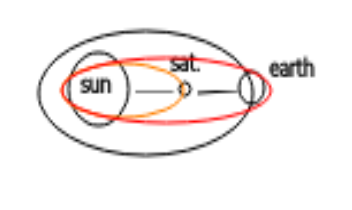
\includegraphics{img/put_it_there.png}
\end{center}
\paragraph{} Consider the previous situation, there are mainly two celestial bodies that we consider, the earth and the sun, the black path by Kepler's Law, the path that described the orbit of the earth around  the sun is an ellipse, the sun has a gravitaional field that is constantly pulling the earth towards it, it is the escape velocity of the earth (which is perpendicular to the suface of the planet), but we want to approach to the sun, and therefore every object part of the dyson swarm will have to escape from the earth and orbit around the sun, on orbital mechanics this can be done by using a transitional orbit (the red ellipse), ant the right moment on the right side of the red ellipse close to the earth a burst of energy must to stay in orbit on the sun and additional velocity must be needed to get far enough and stay in orbit, but to be precise, between the sun and the earth there are several phenomena that is currently under study and yet
\begin{equation}
F = ma
\end{equation}
\begin{equation}
v = \frac{G m_1 m_2}{r^2}¸
\end{equation}
	
on each object the main forces that we will consider will be the the gravitational force of the earth overthe  object, and be far enough from the sun the gravitational force this is possible by using making the following model

\paragraph{}


%\paragraph{Todo} ¿How loosely they should be? ¿how to put one object and which conditions about the object are necessary? ¿Orbiting around the sun or a geostationary? ¿How to transfer the energy from each object to another place? if it is not possible, a capacitor/battery? ¿Which would be the design of these objects? ¿how efficient the should be at the task? ¿How long would it takes use/transfer the collected/transfered energy from one place to another?

\paragraph{Maxwell's Equations} as described on \cite{serway_physics_2019} and \cite{fleisch_students_2008} Maxwell's equations are a set of four equations, that have been defined by James Clerk Maxwell more than a century ago\footnote{Originally there were twenty equations but with the help of Olivier Heavisde, and Heinrich Hertz those equations were combined into four that we have today.}, these equations gave us a door to a deeper understanding of the universe: laws of physics, that were derived from characters such as Gauss and Faraday. These equations help us describe electromagnetic phenomena, and it is one of the reasons why we have today amazing technologies such as computers, radio, wireless internet and among others.
\begin{equation}
	\nabla \cdot D = \rho_V
\end{equation}
\paragraph{}The first equation is known as Gauss'law, and dictates also that charges of the same sign repel. $D$ is the electric flux density and $\rho_V$ the electric charge density.
\begin{equation}
	\nabla \cdot B = 0
\end{equation}
\paragraph{} the second one is Gauss law of magnetism, and dictates that magnetic monopoles do not exists, here $B$ is the magnetic field.
\begin{equation}
	\nabla \times E = -\frac{\partial B}{\partial t}
\end{equation}
\paragraph{}Known as Faraday's Law, this equation describes how a magnetic field over time can produce an electric field.
\begin{equation}
	\nabla \times H = \frac{\partial D}{\partial t} + J
\end{equation}
\paragraph{} Ampére's Law, this equation describes how electromagnetic fields can be generated by changes in time of the electric flux density or by an electric current density $J$.
\paragraph{} Electromagnetic pehonema is a too wide topic, and certainly these equations are difficult to solve, several numerical methods have been applied depending on the geometry of the problem, such as finite element and finite difference, I will choose to model one electromagnetic phenomena (which I'm not sure at the moment but here are some topics/ideas):

\paragraph{} I will attempt to model and use finite difference\cite{monk_finite_2003} or other numerical methods\cite{mismar_numerical_2017}, compare the results, and verify which one is better, simpler and accurate, and in the process learn more about this phenomena.

\paragraph{About the computation}

\paragraph{About the expected results}

\bibliographystyle{unsrt}
\bibliography{bibliography}

\end{document}